\section{Differentiation}

%% Returning to the problem in first section, we want to answer the question of how fasr x is moving at time 2 .

%% As we saw in figure, we can estimate this by taking closer and closer time and distance measurements,,,

%% We can formalize with a limit


\begin{defn}[Definition of the Derivative]\label{DifDef}
	We say that a function $f$ is \emph{differentiable at $a$} if
	\begin{equation}
		f'(a)\coloneqq\lim\limits_{h\to 0}\frac{f(a+h)-f(a)}{h} \text{ exists}.
	\end{equation}
	We call $f'(a)$ the derivative of $f(x)$ at $a$. If $f$ is differentiable at every point it is defined, we say that $f$ is differentiable and call $f'$ the derivative of $f$.
\end{defn}
\begin{rem}
Alternatively, we may write the derivative of $f$ as $\diff{f}{x}(a)$ or $\diff{}{x}\Big(f(x)\Big)$. Here, $\diff{}{x}$ tells us to take the derivative of $f$.
\end{rem}
Let's unpack this definition. Recall that we can write the formula for a line between two points $(x_1, y_1)$ and $(x_2, y_2)$ as
\[
y_2 - y_1 = m(x_2-x_1)
\]
where $m$ is the slope. In this case, we can calculate the slope of this line as
\[
m = \frac{\Delta y}{\Delta x} = \frac{y_2 - y_1}{x_2 - x_1}
\]
which is the change in $y$ divided by the change in $x$. Substituting this into the point-slope formula, we see that
\[
y_2-y_1 = \underbrace{ \left( \frac{\Delta y}{\Delta x} \right) }_{m}(x_2-x_1).
\]

Now looking at \cref{DifDef}, we see that the quotient
\[
\frac{f(a+h)-f(a)}{h}
\] describes the slope of a line between the points $(a, f(a))$ and $(a+h, f(a+h))$, and we want to see what happens to this quotient as $h$ approaches 0.

\begin{center}
	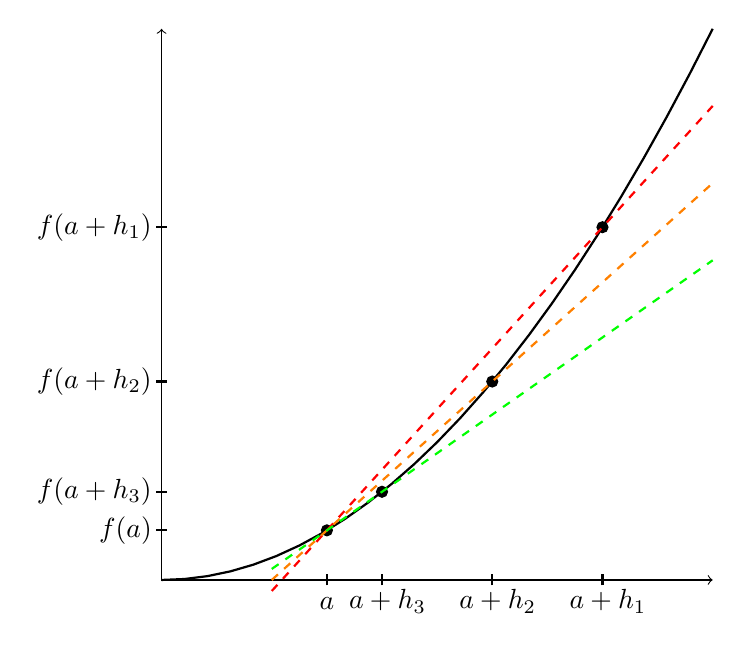
\begin{tikzpicture}[scale=0.7]
		\draw [<->] (10,0)-- (0,0) -- (0,10);
		\draw[thick, domain=0:10] plot (\x, {.1*\x*\x});
		\draw [thick] (3,-0.1)--(3,0.1);
		\node at (3,-0.15) [below] {$a$};
		\draw [thick] (8,-0.1)--(8,0.1);
		\node at (8.1,0) [below] {$a+h_1$};
		\draw [thick] (6,-0.1)--(6,0.1);
		\node at (6.1,0) [below] {$a+h_2$};
		\draw [thick] (4,-0.1)--(4,0.1);
		\node at (4.1,0) [below] {$a+h_3$};

		\draw [thick] (-0.1, 0.9)--(0.1, 0.9);
		\node at (0,0.9) [left] {$f(a)$};
		\draw [thick] (-0.1, 6.4)--(0.1, 6.4);
		\node at (0,6.4) [left] {$f(a+h_1)$};
		\draw [thick] (-0.1, 3.6)--(0.1, 3.6);
		\node at (0,3.6) [left] {$f(a+h_2)$};
		\draw [thick] (-0.1, 1.6)--(0.1, 1.6);
		\node at (0,1.6) [left] {$f(a+h_3)$};

		\draw [fill=black] (3, 0.9) circle [radius=0.1];
		\draw [fill=black] (8, 6.4) circle [radius=0.1];
		\draw [fill=black] (6, 3.6) circle [radius=0.1];
		\draw [fill=black] (4, 1.6) circle [radius=0.1];
		\draw[dashed, red, thick, domain=2:10] plot (\x, {1.1*\x-2.4});

		\draw[dashed, orange, thick, domain=2:10] plot (\x, {0.9*\x-1.8});

		\draw[dashed, green, thick, domain=2:10] plot (\x, {0.7*\x-1.2});


	\end{tikzpicture}
\end{center}

The picture above shows that as $h$ decreases, $\frac{f(a+h)-f(a)}{h}$ begins to resemble the slope of the line tangent to $f(x)$ at $a$. This shows us that the derivative gives us information about the \emph{rate of change} of a function.\\

Motivated by the above picture, we see that if we let $x=a+h$, then our definition of the derivative is equivalent to the following one.

\begin{defn}[Alternative Definition of the Derivative]
	A function $f(x)$ is differentiable at $a$ if
	\begin{equation}\label{AltDifDefEq}
		\lim\limits_{x\to a}\frac{f(x)-f(a)}{x-a}\ \text{exists.}
	\end{equation}
	As before, we denote the value of this limit by $f'(a)$ or $ \diff{f}{x}(a)$.
\end{defn}
\begin{rem}
  Borrowing the notation above, we can write $\Delta f = f(x) - f(a)$ and $\Delta x = x-a$, so that  \eqref{AltDifDefEq} above becomes
  \[
	\lim\limits_{x\to a}\frac{\Delta f}{\Delta x} = \diff{f}{x}(a).
  \]
\end{rem}

%% Example here

Instead of taking the derivative at every single point $a$ that we're interested in, we can try to write the derivative of a function $f(x)$ as another function instead of fixing some point $a$! We can try an example of this.

\begin{exmp}
  From algebra and geometry, we know that a circle with radius $r$ has area $\pi r^2$. What would we do if we wanted to know how quickly the area of the circle would change if we changed our radius. In this case, we write the area function as $A(r) =  \pi r^2$. This time we use the definition of the derivative (\cref{DifDef}) using a variable $r$ for our radius instead of a single point $a$. Therefore, we can attempt to write the derivative $A'(r)$ as
  \[
  A'(r) = \lim\limits_{h\to 0}\frac{A(x+h)-A(x)}{h}.
  \]
  Using our familiar algebra rules, we can show that $A(r+h) = \pi(r+h)^2 = \pi(r^2 + 2rh + h^2) = \pi r^2 + 2\pi rh + \pi h^2$. Therefore, we can rewrite this limit as
  \begin{align}
  A'(x) & = \lim\limits_{h\to 0}\frac{\pi r^2 + 2\pi rh + \pi h^2 - \pi r^2}{h} =  \lim\limits_{h\to 0}\frac{2\pi rh + \pi h^2}{h}\\
  & = \lim\limits_{h\to 0}\frac{h(2\pi r + \pi h)}{h} = \lim\limits_{h\to 0} 2\pi r + \pi h = 2\pi r.
  \end{align} This shows us that the area of a circle of radius $r$ changes at a rate $2\pi r$. We can see this idea geometrically in ()  One thing that should stand out is that this is the same formula as the circumference $C(r)$ of the circle! Therefore, we showed that
  \[
  \diff{A}{r} = C(r).
  \]  In words, this means that the derivative of the area of a circle with radius $r$ is its circumference! We probably wouldn't have noticed this pattern if we tried to find this derivative for specific points one by one.
\end{exmp}

%% Add figure for this circle with $h$


This technique is useful in a lot more cases, so we'll try to generalize this idea a bit. If we have a function $f(x)$ and can find another function that gives us the derivative of $f$ at any point $x$, we simply call it \emph{the derivative of $f$} (without mentioning a specific point). Keeping our notation consistent, we'll write this function as $f'(x)$ or $\diff{f}{x}$! This can be a little confusing at first, but the point is that the derivative of $f$ at a point $a$ is a number $f'(a)$, and the derivative of $f$ is another function $f'$.

When we write it in this way, we can find that the derivative as we defined it has some very nice properties which will make the actual process computing derivatives much easier. You'll notice that several of the properties shown below resemble properties of limits which makes sense since we defined the derivative in terms of limits. These properties also harken back to the limit properties of continuous functions and later, we'll see that all differentiable functions are also continuous.

\subsection{Differentiation Rules}

%% Flesh out this section. Consider moving things around!! Maybe find more indepth examples and exapnd on expositon

As one might expect, using the definition of the derivative on each and every problem we encounter is tedious, boring, and generally uneventful. In order to get around this, we'll develop some tricks for computing derivatives easily using the derivatives of more `elementary' functions.

\begin{prop}[Scalar multiplication and Sum Rules]\label{SMultSumDiff}
	If $f$ and $g$ are differentiable at $a$ and  $c$ is any real number, then $f+g$ and $c\cdot f$ are differentiable at $a$. Moreover,
	\begin{align}
		 (f+g)'(a)&=f'(a)+g'(a)\ \text{and}\\
		  (c\cdot f)'(a)&=c\cdot f'(a).
	\end{align}
\end{prop}
\begin{proof}
We start with the definition of the derivative and through a short computation see that
\begin{align*}
	\lim\limits_{x\to a}\frac{(f+g)(x)-(f+g)(a)}{x-a}&=	\lim\limits_{x\to a}\frac{f(x) +g(x)-f(a)-g(a)}{x-a}\\
	&=\lim\limits_{x\to a}\frac{f(x)-f(a)+g(x)-g(a)}{x-a}\\
	&=\lim\limits_{x\to a}\frac{f(x)-f(a)}{x-a}+\lim\limits_{x\to a}\frac{g(x)-g(a)}{x-a}\\
	&=f'(a)+g'(a).
\end{align*}
Therefore the derivative $(f+g)'(a)$ exists and equals $f'(a)+g'(a)$. A similar computation shows that $(cf)'(a)=c\cdot f'(a)$.
\end{proof}

\begin{thm}[Product Rule]
	If $f$ and $g$ are differentiable at $a$, then $f\cdot g$ is differentiable at $a$ and \begin{equation}
		(f\cdot g)'=f'(a)\cdot g(a)+f(a)\cdot g'(a).
	\end{equation}
\end{thm}

\begin{thm}[Reciprocal Rule]
If $f(x)$ is differentiable at $a$ and $f(a)\neq 0$, then $g(x)=\frac{1}{f(x)}$ is differentiable at $a$ and
\begin{equation}
g'(a)=-\frac{f'(a)}{f(a)^2}.
\end{equation}
\end{thm}

\begin{cor}[Quotient Rule]
	If $f$ and $g$ are differentiable at $a$ and $g(a)\neq 0$, then $Q(x)=\frac{f(x)}{g(x)}$ is differentiable $a$ and
	\begin{equation}
		Q'(a)=\frac{f'(a)g(a)-f(a)g'(a)}{g(a)^2}.
	\end{equation}
\end{cor}

%% Add the chain rule!!

Now that we have all these rules of differentiation, let's see how we can find the derivatives of a common class of functions.

\begin{quest}
	What is the derivative of a polynomial function
	\begin{equation}
		f(x)=a_nx^n+a_{n-1}x^{n-1}+\dotsb+ a_1x+a_0,
	\end{equation}
	where $n=$ is a positive integer and each $a_i$ is any number?
\end{quest}

Let's start with the simple case where our function is constant.

\begin{prop}
The derivative of a constant function $f(x) =c$ is 0.
\end{prop}

\begin{proof}
If $f$ is constant, then $f(x + h) = f(x) = c$. Therefore,
\[
f'(x) = \lim\limits_{h\to 0} \frac{f(x+h)-f(x)}{h} = 0.
\]
\end{proof}

Moving onto the non-constant polynomials, the scalar multiplication and sum rules from above (\label{SMultSumDiff}) tell us that we only need to be able to find the derivative of each $x^k$ to find the derivative of $f(x)$.

\begin{prop}[Power Rule]\label{PowRule}
	If $f(x)=x^n$ for any non-zero number $n$, then the derivative of $f$ is  $f'(x)=nx^{n-1}$.
\end{prop}
\begin{proof}
	We start with the definition of the derivative and substitute in our function $f$ i.e.
	\begin{equation}
		\lim\limits_{h\to 0}\frac{f(x+h)-f(x)}{h}
=	\lim\limits_{h\to 0}\frac{(x+h)^n-x^n}{h}.
	\end{equation}
	Using the fact that \begin{equation}
		(a+b)^n=\sum^n_{k=0} \binom{n}{k}a^{n-k}b^k=a^n+na^{n-1}b+ \frac{n(n-1)}{2!}a^{n-2}b^2+\dotsb+b^n,
	\end{equation}
	where $\binom{n}{k}=\frac{n!}{k!(n-k)!}$,
	we calculate the limit as follows:
	\begin{align}
		\lim\limits_{h\to 0}\frac{(x+h)^n-x^n}{h}&=\lim\limits_{h\to 0}\frac{(x^n+nx^{n-1}h+ \frac{n(n-1)}{2!}x^{n-2}h^2+\dotsb+h^n)-x^n}{h}\\
	&=\lim\limits_{h\to 0}\frac{nx^{n-1}h+ \frac{n(n-1)}{2!}x^{n-2}h^2+\dotsb+h^n}{h}\\
	& =\lim\limits_{h\to 0} \left[ nx^{n-1}+ \frac{n(n-1)}{2!}x^{n-2}h+\dotsb+h^{n-1}\right] .
	\end{align}
Using the additive and multiplicative properties of limits, we see that
\begin{equation}
	f'(x)=\lim\limits_{h\to 0} \left[nx^{n-1}+ \frac{n(n-1)}{2!}x^{n-2}h+\dotsb+h^{n-1}\right]=nx^{n-1},
\end{equation}
which proves the theorem.
\end{proof}

%% Add proving that the derivative of a constant is zero to the exercises

\begin{exmp}
	Using the power rule, find the derivative of $f(x)=x^2+3x$.
\end{exmp}

%% Finish this example


There are other useful derivative formulas that one should know when doing and learning calculus.

\begin{prop}\label{SinCosExpDif}
  The functions $\sin(x), \cos(x)$ and $e^x$ are differentiable.
  \begin{enumerate}
\item The derivative of $\sin(x)$ is $\cos(x)$,
\item the derivative of $\cos(x)$ is $-\sin(x)$,
\item the derivative of $e^x$ is $e^x$, and
\item the derivative of $\ln(x)$ is $\frac{1}{x}$.
\end{enumerate}
\end{prop}
The proofs for the first two parts rely on the following additive identities of trigonometry:
\begin{align}
   \sin(a+b)&=\sin(a)\cos(b)+\cos(a)\sin(b),\\
   \cos(a+b)&=\cos(a)\cos(b)-\sin(a)\sin(b),
\end{align}
and using the following limit identities,
\begin{equation}
  \lim\limits_{x\to 0}\frac{\cos(x)-1}{x}=0 \text{ and } \lim\limits_{x\to 0}\frac{\sin(x)}{x} =1.
\end{equation}
We'll leave the proof of the first two as an exercise, and we'll prove the third and fourth later when we do implicit differentiation.

Now that we understand how to differentiate function like $x^2$ or $\sin(t)$ as well as their sums, products, and quotients, we can begin to tackle a number of problems. But we've yet to answer how we can differentiate \emph{compositions} of functions like $\sin(t^2)$ or $\cos^3(t) + e^{2t}$. That is, we want to understand how we can differentiate functions within other functions. The first step of this is identifying what is a composition of functions. Say we're given the function $\sin(t^2)$ as above. We can clearly see that this is made up of $t^2$ and the familiar $\sin(x)$. To clarify this notation, we write $f(x) = \sin(x)$ and $g(t) = t^2$.  This way, we can see that choosing $x = g(t)$ allows us to write
\[
f(x) = f(g(t)) = f(t^2) = \sin (t^2).
\]
This still doesn't answer the question of differentiation. Let's set up this question more abstractly. Say we have any function $f(x)$ and another function $g(t)$, then our goal is to find the derivative of its composition,
\[
(f\circ g)'(t) = \frac{df}{dt}.
\]
Going back to most basic idea behind the derivative, we know that $f'(x) = \diff{f}{x}$ tells us the rate of change of $f$ as we move near $x$. Therefore, the derivative $f'(g(t))$ should tell us the rate of change near $g(t)$, but since $g$ itself is a function, we must account for the change in $g(t)$ near $t$ i.e. $\diff{g}{t}$. Since $g$ is acting as our input $x$, we can write its derivative as $\diff{x}{t}$.

DONT DO THIS YOURseLF
\[
\diff{f}{t} = \diff{f}{x} \diff{x}{t}.
\]

Handwavely, but the equation is ...

Write as proposition.

\begin{prop}[The Chain Rule]
If $f$ is differentiable at $g(t)$ and $g$ is differentible at $t$, then the derivative of $f\circ g$ is
\[
(f\circ g)'(t) = g'(t)\cdot f'(g(t)).
\]
\end{prop}
\begin{rem}
I often remember this as `the derivative of the inside function times the outside function'.
\end{rem}
%%% ive sin and cos as exercise with the trig rule and limit rule as hints

%% Differentiation Exercises

\begin{exmps}

Compute the derivative $f'(x)$ for the following functions:
\begin{enumerate}[label=\textbf{Example A.\arabic*.}]
  \addtolength{\itemindent}{2.5cm} % move right
  \item \label{DifEA1} $f(x) = x^5+2x+1$,
  \item \label{DifEA2} $f(x) = \sin^3(x)=\big(\sin(x)\big)^3$,
  \item \label{DifEA3} $f(x) = x^3\sin(x)$,
  \item \label{DifEA4} $f(x) =\frac{5x}{x^2+1}$,
  \item \label{DifEA5} $f(x) = e^{6x}$
  \item \label{DifEA6} $f(x) = x^2e^{2x}$
  \item \label{DifEA7} $f(x) = \frac{1}{x^2}$
  \item \label{DifEA8} $f(x) = e^{-6x}\ln(x)$
\end{enumerate}

\textbf{Example A.1.}

Since we're differentiating a sum, we can take the derivative of each of its parts! Using the power rule (\href{PowRule}), we see that the derivative of $x^5$ is $5x^4$, the derivative of $2x$ is $2$ and the derivative of $1$ is 0. This means that the derivative of $x^5 + 2x + 1$ is given by $5x^4 + 2$.

\textbf{Example A.2.}

This problem is an application of the chain rule (add citation) and the power rule! Using the $\sin(x)$ as the `inside' function ($g(x)$) and $x^3$ as the `outside' function $(f(x))$. Starting with the `outside' function $f$ we use the power rule to show
\[
f(x) = x^3 \xrightarrow{\diff{}{x}} f'(x) = 3x^2.
\] by the power rule. Similarly, the derivative of $g(x) = \sin(x)$ is $g'(x) = \cos(x)$ by \cref{SinCosExpDif}. Following the chain rule formula, we can compute $f'(g(x)) = 3 \sin^2(x)$. Therefore, we write the derivative as $3\cos(x)\sin^2(x)$.

%% Make align for the derivative $\diff{}{x}$ over arrow?
\textbf{Example A.3.}

\textbf{Example A.4.}

\textbf{Example A.5.}

\textbf{Example A.6.}

\textbf{Example A.7.}

\textbf{Example A.8.}

\end{exmps}

The derivative is also useful for answering questions about the average rate of change as well as the maxima and minima.


\subsection{Differentiation Theorems}

\begin{thm}[Rolle's Theorem]
Suppose $f$ is continuous on a closed interval $[a,b]$ and differentiable on the open interval $(a,b)$ and $f(a)=f(b)$, then there is some point $c\in [a,b]$ such that $f'(c)=0$.
\end{thm}

With Rolle's theorem, we can define the following theorem which allows us to relate the secant lines discussed earlier with the derivative.
\begin{thm}[Mean Value Theorem]\label{MVTD}
Suppose $f$ is continuous on a closed interval $[a,b]$ and differentiable on the open interval $(a,b)$, then there is some point $c$ in $[a,b]$ such that
\begin{equation}
	f'(c)=\frac{f(b)-f(a)}{b-a}.
\end{equation}
\end{thm}
\begin{proof}
Let $g(x)=f(x)-\frac{f(b)-f(a)}{b-a}(x-a)$. The function $g$ is differentiable with $g(a)=f(a)$ and $g(b)=f(b)$. Using differentiation rules described earlier,
\begin{equation}
	g'(x)=f'(x)-\frac{f(b)-f(a)}{b-a}.
\end{equation}
Therefore, we can apply Rolle's theorem and see that there is some $c$ such that $g'(c)=0$, so
\begin{equation}
	f'(c)=\frac{f(b)-f(a)}{b-a}.
\end{equation}
\end{proof}

Essentially, this theorem states that the secant line of $f$ at the points $a$ and $b$ has the same slope as the derivative $f$ at some point $c$ or \emph{the average rate of change on $[a,b]$ is realized as the instantaneous rate of change at a point $c$ in $[a,b]$}.

%%%%% Figure showing what this looks like %%%
